\section{Actions on the snapshot}

Any high-level language will be somehow compiled or interpreted to run
as machine instructions. The instruction set architecture (ISA) are
often a relatively small set of opcodes matching to the assembly
language. An ISA includes:
\begin{itemize}
\item Arithmetic (such as \emph{add} and \emph{sub})
\item Logic instructions (such as \emph{and}, \emph{or} and \emph{not})
\item Data instructions (such as \emph{move}, \emph{input}, \emph{output}, \emph{load}, and \emph{store})
\item Control flow instructions (such as \emph{goto}, \emph{if ... goto}, \emph{call}, and \emph{return})
\end{itemize}

Arithmetic and logic instructions are simply pure CPU operations. We
are insterested in instructions touching the main memory and
instructions controlling them.

The language we allow abstracts away the CPU operations and narrows
down the operations to a set of movers, i.e.\ loading from and storing
to the main memory and operations related to thread
bookkeeping. Operations like $x:=y$ will be considered in our model as
a 2-steps (atomic) operation composed of a load (of $y$) and a store
(of $x$). Operations like $x:=3*y$ will be considered as a 3-steps
operation composed of a load (of $y$), a pure CPU operation, and a
store (of $x$).

Abstracting away all instructions gives us a set of atomic movers from
main memory (the Loads) and a set of movers to main memory (the
Stores). We can abstract away the data itself. We will keep the
control flow instructions to reflect them in the job types.

\bigskip\noindent%
For the shared variables, we have then 2 actions: read and write. 
\begin{itemize}
\item \underline{Read}: \\%
  \begin{minipage}{0.5\linewidth}
  Atomic action which we divide in two steps. The first step is a
  request for reading, which put a pair %
  \tikz[baseline=(x)]{\node[pair,scale=0.6](x){T$_i$\nodepart{lower}R};} %
  in the associated set, where T$_i$ is the reading thread. The second step is to remove the pair (and perform the read atomically).%    
  \end{minipage}
  \begin{minipage}{0.5\linewidth}
    \begin{center}
      \begin{tikzpicture}
        \node[mystate=blue!50,inner sep=1pt](s1){S$_1$};
        \node[mystate=blue!50!green](s1t) at (1cm,-10mm){};
        \node[mystate=green,inner sep=1pt](s2) at (0,-20mm){S$_2$};

        \draw[->] (s1) -- (s1t) node[pos=0.3,right,scale=0.7]{T$_i$: Read X};
        \draw[->] (s1t) -- (s2) node[pos=0.7,right,scale=0.7]{atomic};

        \begin{scope}[shift={(21mm,0mm)}]
          \node[fill=yellow,inner sep=1pt,circle](x){X};
          \node[ellipse,fill=yellow,minimum width=25mm, minimum height=10mm](set) at +(10mm,-15mm){};
          \filldraw[yellow] (x.-130) to[out=-50,in=20] (set.160) -- (set.90) to[out=180,in=-100] (x.-10) -- (x.-40) -- (x.-90);
          \node[pair,scale=0.7,left=1mm of set.center]{T$_i$\nodepart{lower}R};
          \node[right=1mm of set.center]{...};
        \end{scope}
      \end{tikzpicture}
    \end{center}
  \end{minipage}
  % 
\item \underline{Write}: \\%
  Similar to the read but a pair %
  \tikz[baseline=(x)]{\node[pair,scale=0.6](x){T$_j$\nodepart{lower}W};} %
  is inserted in the access set.
\end{itemize}

\bigskip\noindent%
For the mutexes, we allow 3 actions: lock, unlock and try-lock. Each
mutex is a special shared variable which value is either \emph{taken}
or \emph{free}.
\begin{itemize}
\item \underline{Lock}: (or grab, take, request, ...) \\%
  \begin{minipage}{0.6\linewidth}
    The lock action starts by moving the current thread to a temporary
    state. If the mutex is free, the variable is atomically updated to
    taken, and the thread moves out of the temporary state. If the
    mutex is taken, the thread doesn't exit the temporary state. Note
    that this models well the fact that only one can succeed in
    locking the mutex.
  \end{minipage}
  \begin{minipage}{0.4\linewidth}
    \begin{center}
      \begin{tikzpicture}
        \node[mystate=blue!50,inner sep=1pt](s1){S$_3$};
        \node[mystate=blue!50!green](s1t) at (1cm,-10mm){};
        \node[mystate=green,inner sep=1pt](s2) at (0,-20mm){S$_4$};
        
        \draw[->] (s1) -- (s1t) node[pos=0.3,right,scale=0.7]{T$_i$: Lock L$_1$};
        \draw[->] (s1t) -- (s2) node[pos=0.7,right,scale=0.7]{atomic update};
        
        \draw[->] (s1t) .. controls +(45:5mm) and +(-45:5mm) .. (s1t) node[midway,right,scale=0.7]{if taken};
      \end{tikzpicture}
    \end{center}
  \end{minipage}
  %
\item \underline{Unlock}:\\%
  If the mutex was taken, resetting it to free will release the mutex,
  allowing other blocked threads to compete for the mutex. If it was
  free, nothing happens.\daz{But still something fishy here...}
  % 
\item \underline{Lock with timer}: (or try-lock) \\%
  \begin{minipage}{0.6\linewidth}
    Behaves like the lock, but the request can timeout and the thread
    moves back to its original state.
  \end{minipage}
  \begin{minipage}{0.4\linewidth}
    \begin{center}
      \begin{tikzpicture}
        \node[mystate=blue!50,inner sep=1pt](s1){S$_3$};
        \node[mystate=blue!50!green](s1t) at (1cm,-10mm){};
        \node[mystate=green,inner sep=1pt](s2) at (0,-20mm){S$_4$};
        
        \draw[->] (s1) -- (s1t) node[pos=0.3,right,scale=0.7]{T$_i$: Lock L$_1$};
        \draw[->] (s1t) -- (s2) node[pos=0.7,right,scale=0.7]{atomic update};
        
        \draw[->] (s1t) .. controls +(45:5mm) and +(-45:5mm) .. (s1t) node[midway,right,scale=0.7]{if taken};
        \draw[->] (s1t) to[out=180,in=-90] (s1) node[midway,left,scale=0.7]{timeout};
      \end{tikzpicture}
    \end{center}
  \end{minipage}
  % 
\end{itemize}


\bigskip\noindent%
For a thread, we allow creation and termination. We also allow a thread to wait for another one.\daz{or several other ones?}
\begin{itemize}
\item \underline{Creation}: \\%
  We add another thread entity to the collection with a new job type,
  a start state, some initialization for the locals. Note that all of
  the initialization steps can be parametrized.%
  \daz{multiple creation and join temporarily on hold}
  % 
\item \underline{Join(id)}:\\%
  A 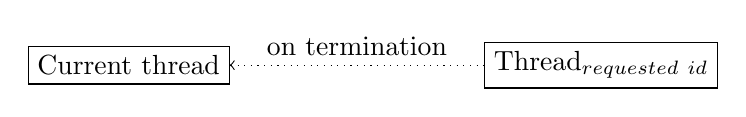
\begin{tikzpicture}[baseline=(jt1.base)]
    \node[draw](jt1) {Current thread};
    \node[draw](jt2) at (6,0){Thread$_{requested\ id}$};
    \draw[dotted,<-] (jt1.east) -- (jt2.west) node[midway,above,sloped]{on termination};
  \end{tikzpicture} %
  association is added and the calling thread goes to an intermediary
  sleeping state.
%
\item \underline{Termination}:\\%
  The thread is removed from the collection.\daz{Its id is not
    recylcled. Other threads might still try to communicate with it,
    which should result in some sort of failure}. If an on-termination
  link was present, notification is send to all other joined threads,
  moving them out of their intermediary sleeping state.
  %
  \ignore{
  \item \underline{Multiple Creation}: \\%
    A thread can create an arbitrary number of other threads. This is
    often bounded and parametrized.%
    \daz{afaik, noone writes code with an eventually infinite loop}
    % 
  \item \underline{Multiple Join}:\\%
    We need a multiple join for the abstraction, since we have the multiple create.\daz{todo}
    % 
  }%
\end{itemize}


For the condition variables:\daz{todo}
\begin{itemize}
\item \underline{Wait}%: \\%
\item \underline{Signal}%: \\%
\item \underline{Broadcast}%:\\%
\end{itemize}
